\documentclass[a4paper,10pt]{article}

\usepackage[english,activeacute]{babel}
\usepackage[english]{layout}
\usepackage{amsfonts,amsmath,amssymb,amsthm}
\usepackage[dvips]{graphicx}
\usepackage{color}
\usepackage{subfig}
\usepackage{colonequals}
\usepackage[latin1]{inputenc}
\usepackage{url}
\usepackage{epsfig}
\usepackage{dsfont}

\usepackage{algorithm}
\usepackage{algorithmic}
\usepackage{setspace}
\usepackage{afterpage}
%\usepackage{showkeys}
% \usepackage{mathptmx}      % use Times fonts if available on your TeX system
% \usepackage{latexsym}

%\usepackage[left=1.2in,right=1.2in]{geometry}

% \graphicspath{{../iccv09/}}

\newcommand{\ma}[1]{\boldsymbol{#1}}
\newcommand{\tras}[1]{#1^{\mathrm{T}}}
\newcommand{\herm}[1]{#1^{\mathrm{H}}}
\newcommand{\con}[1]{#1^{\mathrm{*}}}
\newcommand{\E}{\mathds{E}}
\newcommand{\tech}[1]{\overline{#1}}
\newcommand{\nspace}{\!\!\!\!}
\newcommand{\nmbr}[1]{\oldstylenums{#1}}

\newcommand{\eg}{\emph{e.g}. } \newcommand{\Eg}{\emph{E.g}. }
\newcommand{\ie}{\emph{i.e}. } \newcommand{\Ie}{\emph{I.e}. }
\newcommand{\cf}{\emph{c.f}. } \newcommand{\Cf}{\emph{C.f}. }
\newcommand{\etc}{\emph{etc}. } \newcommand{\vs}{\emph{vs}. }
\newcommand{\wrt}{w.r.t\onedot } \newcommand{\dof}{d.o.f. }
\newcommand{\etal}{\emph{et al}. }

\newcommand{\R}{\mathds{R}}
\newcommand{\sign}{\mathrm{sign}}
\newcommand{\eps}{\varepsilon}
\newcommand{\To}{\longrightarrow}
% \newcommand{\II}{1{\hskip -2.5 pt}\hbox{I}}

% c++ code
\usepackage{listings}
\usepackage{xcolor}
\usepackage{textcomp}
\definecolor{listinggray}{gray}{0.9}
\definecolor{lbcolor}{rgb}{0.9,0.9,0.9}
\lstset{
	backgroundcolor=\color{lbcolor},
	tabsize=4,    
%  rulecolor=,
	language=Matlab,
	basicstyle=\scriptsize\ttfamily,
	upquote=true,
	aboveskip={1.5\baselineskip},
	columns=fixed,
	showstringspaces=false,
	extendedchars=false,
	breaklines=true,
	prebreak = \raisebox{0ex}[0ex][0ex]{\ensuremath{\hookleftarrow}},
	frame=single,
	numbers=left,
	showtabs=false,
	showspaces=false,
	showstringspaces=false,
	identifierstyle=\ttfamily,
	keywordstyle=\color[rgb]{0,0,1}\ttfamily,
	commentstyle=\color[rgb]{0,0.5,0}\ttfamily,
	stringstyle=\color[rgb]{0.627,0.126,0.941}\ttfamily,
	numberstyle=\color[rgb]{0.5, 0.5, 0.5}\ttfamily,
%  \lstdefinestyle{C++}{language=C++,style=numbers}’.
}
%\lstset{
%	backgroundcolor=\color{lbcolor},
%	tabsize=4,
%	language=C++,
%	captionpos=b,
%	tabsize=3,
%	frame=lines,
%	numbers=left,
%	numberstyle=\tiny,
%	numbersep=5pt,
%	breaklines=true,
%	showstringspaces=false,
%	basicstyle=\footnotesize,
%	identifierstyle=\color{magenta},
%	keywordstyle=\color[rgb]{0,0,1},
%	commentstyle=\color{green},
%	stringstyle=\color{red}
%}
	
	
	


\DeclareMathOperator*{\argmin}{arg\,min}
\DeclareMathOperator*{\argmax}{arg\,max}

\newcommand{\nota}[1]{\textcolor{blue}{\textbf{#1}}}
\newcommand{\suggest}[1]{\textcolor{yellow}{#1}}
\newcommand{\add}[1]{\textcolor{green}{#1}}
\newcommand{\remove}[1]{\textcolor{red}{#1}}
\newcommand{\dosdv}[1] {#1}
\newcommand{\uncite}[1] {}
% \newcommand{\tachar}[1]{
% \setbox4=\hbox{\ } \setbox3=\hbox{#1} \hbox{#1} \kern -\wd3 \kern
% -\wd4 \raise 0.3\ht3 \hbox{ \vrule width \wd3 height 0.5pt} }

% \theoremstyle{plain}\newtheorem{theorem}{Theorem}[chapter]
% \theoremstyle{plain}\newtheorem{proposition}{Proposition}[chapter]
% \theoremstyle{plain}\newtheorem{lemma}{Lemma}[chapter]
% \theoremstyle{definition}\newtheorem{definition}{Definition}[chapter]

% New definition of square root:
% it renames \sqrt as \oldsqrt
\let\oldsqrt\sqrt
% it defines the new \sqrt in terms of the old one
\def\sqrt{\mathpalette\DHLhksqrt}
\def\DHLhksqrt#1#2{%
\setbox0=\hbox{$#1\oldsqrt{#2\,}$}\dimen0=\ht0
\advance\dimen0-0.2\ht0
\setbox2=\hbox{\vrule height\ht0 depth -\dimen0}%
{\box0\lower0.4pt\box2}}

\title{Temporal consistency in Video NL-Bayes}
\author{}
\date{}

\begin{document}

\maketitle
\abstract{Strategies for achieving temporal consistency in video
NL-Bayes using 2D patches.}

\subsection*{Overview}

NL-Bayes groups similar 2D patches and denoise them jointly with a
Wiener shrinkage operator, by assuming that the prior distribution of
the noiseless group is Gaussian. This approach is able to achieve
high PSNRs, however
\begin{enumerate}
	\item for high noise power the results lack temporal consistency,
		and
	\item it is computationally costly.
\end{enumerate}

In order to tackle both issues, we will try to use motion
information. First to achieve temporal consistent results, and
second to speed-up the search for similar patches by searching
in a smaller area around the motion trajectory.
%
In a first stage, we will forget about the computational cost, and
focus on achieving high quality, temporal consistent results.

\bigskip

\bigskip

\begin{figure}[htpb!]
	\centering
	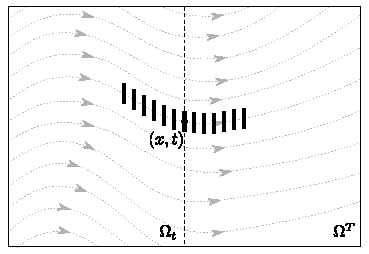
\includegraphics[width=0.33\textwidth]{figs/approach1}%
	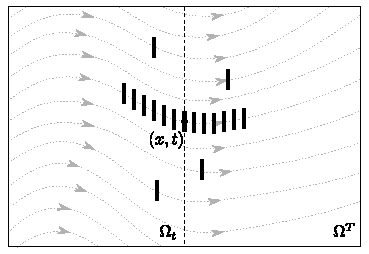
\includegraphics[width=0.33\textwidth]{figs/approach2}%
	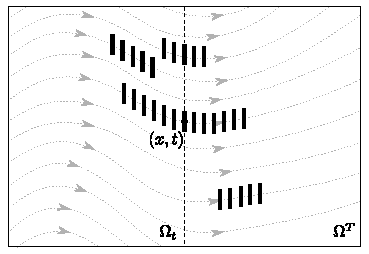
\includegraphics[width=0.33\textwidth]{figs/approach3}
	\caption{Diagrams of three approaches for a 1D video. Motion
	trajectories are represented by the gray doted lines. Patches
	in the patch group for pixel $(x,t)$ are shown as vertical bars.
   From left to right, A1, A2 and A3.}
	\label{fig:3_approaches}
\end{figure}


We propose four strategies. The difference is on how we build the patch 
group $G(x,t)$ of patches similar to the one on $(x,t)$.
By testing these approaches we should evaluate if we can impose temporal 
consistency by manipulating the set of similar patches, which seems to 
be the simplest approach. 
\begin{enumerate}
	\item[\textbf{A0.}] $G(x,t)$ is built by considering similar
		patches in a spatio-temporal region centered at the motion
		trajectory through $(x,t)$. 
	\item[\textbf{A1.}] $G(x,t)$ is built by considering patches in the motion trajectory
		through $(x,t)$. This approach only exploits temporal redundancy. The amount
		of noise reduction will be bounded by the length of the trajectories.
	\item[\textbf{A2.}] $G(x,t)$ is build from the motion trajectory through $(x,t)$,
		plus some similar patches which are not require to lie on the motion
		trajectory.
	\item[\textbf{A3.}] $G(x,t)$ is build from the motion trajectory through $(x,t)$,
		plus some similar patches which are not require to lie on the motion
		trajectory, toghether with their motion trajectory.
\end{enumerate}

\bigskip

\bigskip


\subsection*{Motion estimation and its reliability}

All the previous approaches rely on an estimate of the motion. Computing a 
reliable motion estimate in the presence of noise is itself a problem.
to compute in the presence of high noise.

We will start by testing optical flow algorithms. We should identify 
algorithms that are less sensitive to noise. Also, we can use some tricks
to reduce the noise level:
\begin{enumerate}
	\item Estimate motion on a zoomed-out version of the image (as a side
		effect, this is good for computational cost)
	\item Apply a temporal filter. If the motion is uniform (no acceleration)
		temporal filtering conmutes with the warping induced by the motion, thus
		corresponding pixels can still be matched. For a short-time temporal
		filter we could gain some noise reduction for motions that have a small
		acceleration. 
	\item Other\dots ?
\end{enumerate}


\bigskip

\bigskip


\subsection*{Work plan}

\begin{enumerate}
	\item Evaluate different optical flow algorithms and their
		robustness to noise. Evaluate the effect of zooming the image
		out and temporal smoothing.
	\item Implement and test approach A0.
	\item Implement and test approach A1.
	\item Implement and test approach A2.
	\item Implement and test approach A3.
\end{enumerate}

\end{document}
